% kobe.Rnw --
%
% Author: laurence kell <lauriekell@gmail.com>

%\VignetteIndexEntry{kobe}
% Meta information - fill between {} and do not remove %
% \VignetteIndexEntry{An R Package for ...}
% \VignetteDepends{reshape, plyr}
% \VignetteKeywords{kwd1, kwd2}
% \VignettePackage{...}

\documentclass[a4paper, 11pt, oldtoc]{artikel1}
\usepackage[onehalfspacing]{setspace}
\usepackage{natbib} \bibliographystyle{plain}
\usepackage{graphicx, psfrag, Sweave}
\usepackage{enumerate}


\begin{document}


%------ Frontmatter ------
\title{Kobe Plotting}
\author{Laurie Kell\footnote{ICCAT}}
\date{June 2012}
\maketitle
\tableofcontents

\section{Introduction}

Scientific Advice within the tuna Regional Fisheries Management Organisations (tRFMOs) is based on a common framework 
(ref). The advice requires estimation of the probabilities of $F \textless F_{MSY}$ and
$B$ \textgreater $B_{MSY}$ for a range of management options, generally a range of total allowable catchs (TAC). Advice is presented as 

\begin{itemize}
 \item a phase plot showing fishng mortality and stock status relevant to management reference points
 \item a pie chart summarising current stock status; and 
 \item a Kobe strategy matrix which summarises the probability of achieving management targets for different management options over time.
\end{itemize}

This requires, a stock assessment, estimates of reference points and projections
In this document we show how R can be used to summarise stock assessment results in the Kobe II format using the R package \texttt{kobe}. 

The package can be loaded with the command:


\section{Input Data}

The package requires a data.frame with columns for stock and fishing mortality relative and columns describing
any scenarios. Data can be read in from different stock assessment outputs using methods 
in other FLR packages; see the section on Stock Assessment Packages for examples.

The basic data needed are time series of $F/F_{MSY}$ and $SSB/B_{MSY}$ (or some other benchmark such as $F_{0.1}$)
for historic and projections. These need to include estimates of uncertainty, e.g. produced by bootstrapping an
assessment or running Monte Carlo Markov Chain simulations. An example data set is


\section{Stock Trends}

\section{Phase plot}

\section{Probabilities}

\section{K2SM}

\section{Assessment Packages}

\begin{Schunk}
\begin{Sinput}
> library(kobe)
> library(ggplot2)
> library(plyr)
> library(reshape)
> ## example data sets
> data(sims)
\end{Sinput}
\end{Schunk}

\begin{Schunk}
\begin{Sinput}
> ggplot(assmt)   + 
+   geom_hline(aes(yintercept=1),col="red",size=2)  + 
+   geom_line( aes(year,stock,group=iter,col=iter))
\end{Sinput}
\end{Schunk}


\begin{figure}
\begin{center}
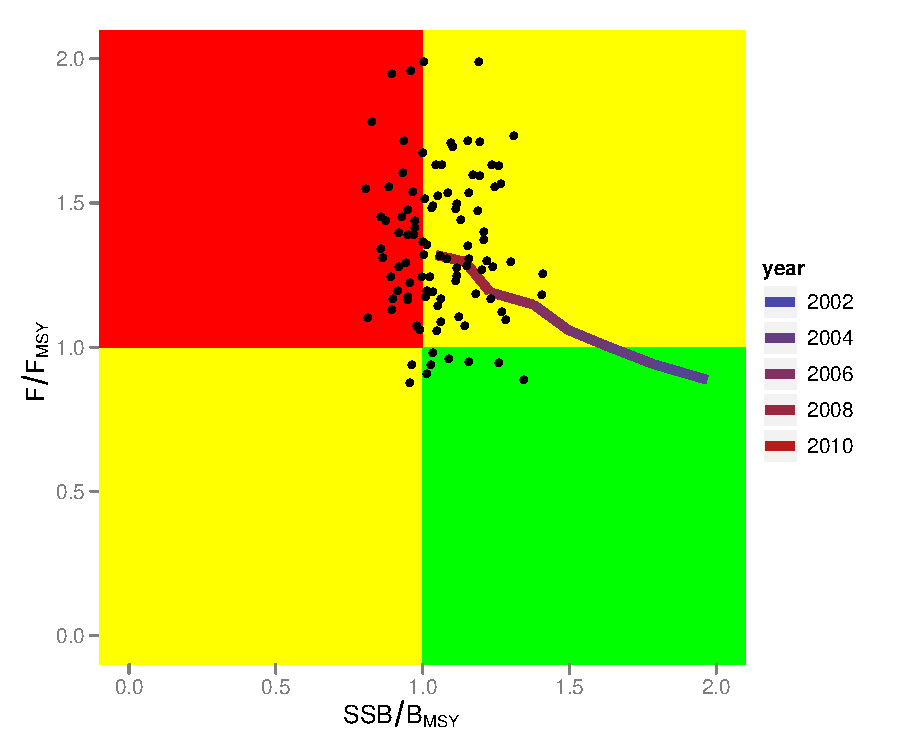
\includegraphics{kobe-005}
\caption{Time series of SSB}
\end{center}
\end{figure}

\begin{figure}
\begin{center}
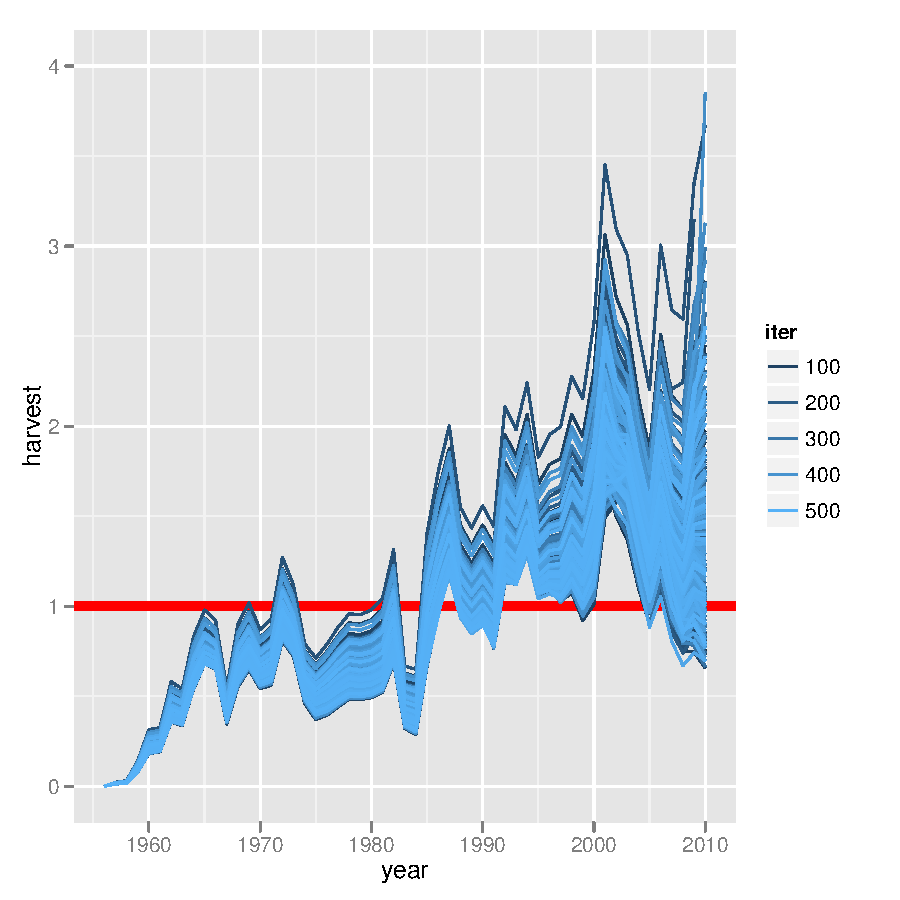
\includegraphics{kobe-006}
\caption{Time series of SSB}
\end{center}
\end{figure}

\begin{figure}
\begin{center}
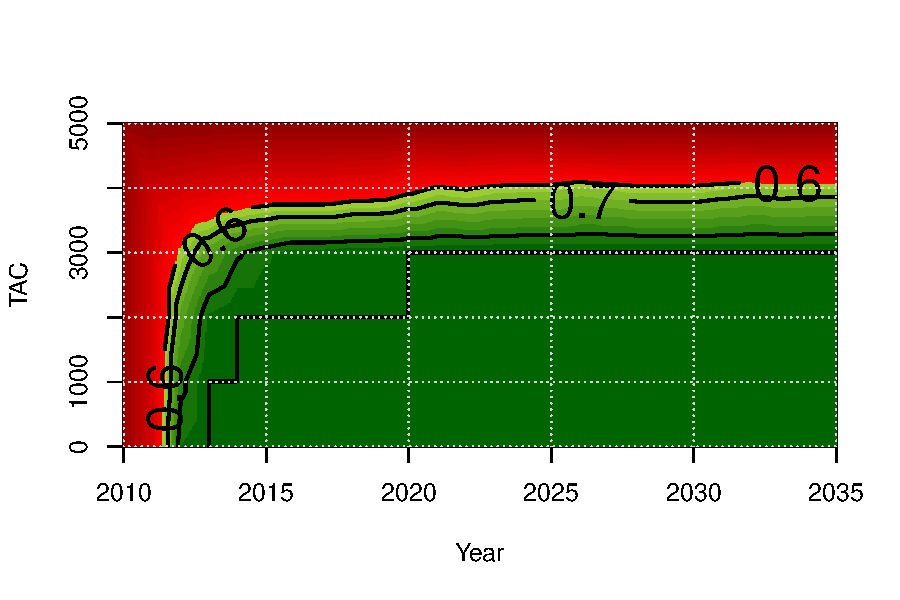
\includegraphics{kobe-007}
\caption{Time series of SSB}
\end{center}
\end{figure}


\section{Implementation}



The plots are implement using three methods, 

The data and code used in this document is in the package {\tt kobe} , which first need to be loaded e.g.


kobe.ts contains a time series of ssb relatuve to $B_{MSY}$ and F relative to $F_{MSY}$ for a historical time series and a projected time series for a range of TACs by iteration.
There is a method kobe that produces the kobe phase, a function that generates the K2SM and a utility function kobeP.

To summarise these data the medians of ssb and havest are calculated, since the data are by iteration

as seen by plotting the data



The trends in SSB and fishing mortality can also be plotted


\section*{Kobe Advice Framework}

The Kobe Advice Framework is based on the Kobe Phase Plot and the Kobe II Strategy Matrix (K2SM). 
The phase plot plots F relative to $F_{MSY}$ against SSB relative to $B_{MSY}$


The four quadrants correspond to

The management objective is to recover the stock and reduce fishing mortality so that the stock is in the green quadrant. Therefore
projections are performed to evaluate the consequences of different TACs e.g. by plotting the median trajectories

This plot does not include the full uncertainty, i.e. the probability of being in the green quadrant for a given TAC in any year.
The function kobeP caculates the various probabilities e.g. 

In addition 


or a matrix


The probabilities can also be plotted as pie charts e.g. if the Commission have a agreed a TAC of x then the expected probabilities over time are given by


\section*{Extended Examples}

In this section show how the basic plots can be enhanced and further analyses conducted.

\subsection*{Mariginal Densities}


\subsection*{Contouring}

\subsection*{Combined Plots}

\subsection*{Alternative K2SMs}

\section*{FLR}

In this section we show the flexibility when assessment methods are implemented as R packages and provide examples of how to using existing assessment packages 
to provide Kobe advice and 

If an assessment model is implemented in R then the inputs and results can easily be processed by R packages, functions and scripts. However most stock assessment 
software relies upon text files for data input therefore many packages now provide R packages to help read these text files into R. Once a data.frame is
available then the examples in the previous section can be used. We then provide some examples of how the code can be extended. 

\section*{Executables}

\subsection*{ASPIC}

ASPIC

\subsection*{VPA2Box}
\subsection*{SS3}
\subsection*{Multifan-CL}

\section*{Further Examples}


\section*{References}

\section*{Appendix}

  \begin{enumerate}
    \item  In support of the SCRS scientific advice, the Executive Summaries within the SCRS annual report which present the results of the stock assessment results should include, when possible: 
    \begin{enumerate}[i)]
      \item A statement characterizing the robustness of methods applied to assess stock status and to develop the scientific advice. This statement should focus on modeling approaches and on assumptions.
      \item Three Kobe matrices, in accordance with the format set out in Annex Table 2:
      \begin{enumerate}[(a)]
         \item A Kobe II strategy matrix indicating the probability of B>$B_{MSY}$ for different levels of catch across multiple years.
         \item A Kobe II strategy matrix indicating the probability of F<$F_{MSY}$ for different levels of catch across multiple years.
         \item A Kobe II strategy matrix indicating the probability of B>$B_{MSY}$ and F<$F_{MSY}$ for different levels of catch across multiple years.
         \item Kobe II strategy matrices to be prepared by the SCRS should highlight in a similar format as shown in Annex Table 2 a progression 
                 of probabilities over 50 \% and in the range of 50-59 \%, 60-69 \%, 70-79 \%, 80-89 \% and ??? 90 \%. 
         \item When the Commission agrees on acceptable probability levels on a stock by stock basis and communicates them to the SCRS, 
                 the SCRS should prepare and include, in the annual report, the  Kobe II strategy matrices using color coding corresponding to these thresholds.
      \end{enumerate}

      \item  A statement concerning the reliability of long term projections period.
      \item   A Kobe plot chart showing
      \begin{enumerate}[(a)]
        \item management reference points expressed as FCURRENT on $F_{MSY}$ (or a proxy) and as BCURRENT on $B_{MSY}$ (or a proxy);
        \item the estimated uncertainty around current stock status estimates;
        \item the stock status trajectory. in accordance with the format set out in Annex Figure 1.
      \end{enumerate}

      \item  A pie chart summarizing the stock status showing the proportion of model outputs that are within the green quadrant of the Kobe plot chart (not overfished, no overfishing), the yellow quadrant (overfished or overfishing), and the red quadrant (overfished and overfishing), in accordance with the format set out in Annex Figure 2.
      \item  An indication of the modeling approaches used by the SCRS to conduct the stock assessment shall be included in the caption and in the corresponding text accompanying the introduction of the matrices and the charts.
      \item  Statements, where needed, reflecting the different opinions expressed regarding the SCRS scientific advice during the endorsement process.
    \end{enumerate}

    \item  The Kobe plot chart described in paragraph 1 should reflect the uncertainties on the estimates of the relative Biomass (BCURRENT on $B_{MSY}$??or its proxy) and of the relative fishing mortality (FCURRENT on $F_{MSY}$ or its proxy), provided that statistical methods to do so have been agreed upon by SCRS and that sufficient data exist to do so.
    \item  The SCRS should review recommendations and templates for the Kobe II strategy matrices, plot and pie charts as laid down in this resolution and should advise the Commission on possible improvements.
    \item  If the Commission adopts alternative reference points, such as limit reference points associated to the precautionary approach, the SCRS should also provide in its annual report versions of the elements described in paragraphs 1 and 2 calculated with respect to these alternative reference points and following the format specified in the same paragraphs.
    \item   The SCRS should indicate in its annual report those cases where the modeling approaches used during the assessment and/or data limitation did not allow for the preparation of the elements mentioned above. 
    \item   The Kobe II strategy matrices are intended to reflect the scientists understanding of the uncertainties associated with their model estimates. Therefore, where models and/or data are insufficient to quantify those uncertainties, the SCRS should consider alternative means of representing them in ways that are useful to the Commission.
    \item   When, due to data limitations, the SCRS is unable to develop Kobe II strategy matrices and associated charts or other estimates of current status relative to benchmarks, the SCRS should develop its scientific advice on fisheries indicators in the context of Harvest Control Rules, if previously agreed upon by the Commission.
    \item   The SCRS should also include in its annual report any other tables and/or graphics that it considers useful to provide advice to the Commission.
    \item   The Commission encourages the SCRS to also include in the detailed reports, where possible, the following additional elements:

    \begin{enumerate}[i)]
      \item a scoring table addressing data completeness and quality with the format set out in Annex Table 1;
      \item information on the by-catches of the different fleet segments and fisheries, as well as other ecosystems considerations.
      \end{enumerate}
  \end{enumerate}

\end{document}
